\chapter*{Introduction Générale}
\label{chap:intro}
\addcontentsline{toc}{chapter}{\nameref{chap:intro}}

\section{Contexte et Motivations}
\label{sec:intro:contexte}
Une décision judiciaire peut être définie soit comme  le résultat rendu par des juges à l'issue d'un procès, ou bien un document décrivant une affaire judiciaire en résumant les faits, les procédures suivies, la solution des juges, et les raisons qui les y ont conduits. \textcolor{red}{UNE DÉCISION JURISPRUDENTIELLE vs. DÉCISION JUDICIAIRE?}. Un corpus de décisions jurisprudentielles ou une jurisprudence\footnote{\url{http://www.toupie.org/Dictionnaire/Jurisprudence.htm}} est par conséquent un ensemble de décisions rendues par les tribunaux et qui représente la manière dont les tribunaux interprètent le droit et les lois pour résoudre un problème juridique donné (type de contentieux). Les décisions sont des documents rédigés par des juges et par conséquence, elles regroupent les éléments de l'affaire\footnote{Depuis le véritable début du contentieux} que ces juges ont retenu comme étant importants à considérer pour prendre leurs décisions sur les prétentions des différentes parties. La compréhension des décisions tourne donc autour des demandes des parties et résultats des juges.

Les décisions judiciaires sont essentielles pour les juristes qui ont l'habitude d'en collecter, sélectionner et analyser pour résoudre les problèmes auxquels ils s'intéressent afin de mieux comprendre \citep{ancel2003expulsion} et anticiper (par ex. les avocats pour leur clients) les décisions des juges. Généralement manuelle, cette analyse rencontre quelques limites. D'abord, l'accès à un corpus exhaustif de décisions est difficile vu l'énorme volume de décisions réparti dans les juridictions (plus de 4 millions de décisions en France par an d'après les chiffres du ministère français de la justice \footnote{\url{http://www.justice.gouv.fr/budget-et-statistiques-10054/chiffres-cles-de-la-justice-10303/}} comme l'illustre le Tableau \ref{tab:intro:nbdecisionstats}). Malgré la disponibilité d'un nombre important de décisions en ligne, les moteurs de recherche juridiques proposent essentiellement des critères à mots-clés. 
\begin{table}[ht]
{
\scriptsize
\begin{center}
\begin{tabular}{|l|c|c|c|c|c|}
\hline
 & \textbf{2010} & \textbf{2011} & \textbf{2012} & \textbf{2013} & \textbf{2014} \\
 \hline
 \textbf{Justice civile} & 2 673 131  & 2 654 179 & 2 647 813 & 2 761 554  & 2 618 374 \\
 \hline
Justice pénale & 1 173 242 & 1 180 586 & 1 251 979 & 1 303 469 & 1 203 339 \\
 \hline
 Justice administrative & 224 787 & 225 608 & 228 680 & 221 882 & 230 477 \\
 \hline
\end{tabular}

\textit{\scriptsize{Source: \url{http://www.justice.gouv.fr/budget-et-statistiques-10054/chiffres-cles-de-la-justice-10303/}}}  
\end{center}
}
\caption{Nombre de décisions prononcées en France par an de 2010 à 2014}\label{tab:intro:nbdecisionstats}
\end{table}

D'autre part, l'analyse manuelle de décisions peut devenir pénible lorsque les documents sont longs et nombreux.  Par ailleurs, la justice est complexe et son langage difficilement compréhensible \citep{cretin2014justicecomplexe} pour permettre aux non-juristes d'estimer le risque judiciaire qu'ils encourent sans l'aide d'un initié en droit. D'une part, une analyse automatisée des décisions jurisprudentielles peut aider des avocats et chercheurs en droit à comprendre l'opinion des juges sur certaines questions. L'exigence pour le profane étant l'exacte pertinence des resources, leur accessibilité, et l'intituivité du processus de leur exploition \citep{narazenko2017legalnlpintro}. D'autre part, elle constitue potentiellement une aide précieuse pour les particuliers et entreprises soucieux de connaitre les chances que leurs requêtes aboutissent en justice.  De telles analyses sont indispensables pour les pratiquants du droit car elles fournissent un ensemble important d'information d'une valeur inestimable dont notamment un aperçu de l'application de la loi. L'extraction automatique d'information pertinente à cette étude aiderait à mieux décrire et organiser les décisions tout en enrichissant les critères de recherche avec par exemple les noms de juges ou les articles de loi. Ce mémoire présente les résultats d'une étude visant à automatiser l'extraction d'information à partir de ces documents afin de faciliter la recherche et les analyses descriptives et prédictives d'un corpus jurisprudentiel. La principale motivation est l'exhaustivité qui passe nécessairement par un traitement rapide et efficace de la grande masse de documents produit par la justice. La question à la base de notre étude est celle de savoir "Comment exploiter un corpus de décisions pour analyser, voire prédire, les décisions des juges sachant que l'interprétation subjective des règles juridiques rend l'application de la loi non déterministe ?". Cette question intéresse de nombreuses entreprises telles que LexisNexis avec son système LexMachina\footnote{\url{https://lexmachina.com}}, et de jeunes startups françaises telles que Predictice\footnote{\url{http://predictice.com}} et CASE LAW ANALYTICS\footnote{\url{http://caselawanalytics.com}}. Afin d'y répondre, nous sommes partis d'une conception théorique considérant la demande ou prétention des parties comme le concept central d'une décision (Figure \ref{fig:intro:demande-central}) et tout autour s'affectent d'autres concepts, notamment, le résultat des juges relatif à cette prétention, le fondement juridique de la prétention ou norme, la catégorisation des prétentions, et ensuite les différentes circonstances factuelles dans lesquelles cette prétention est généralement formulée. 

\begin{figure}[h]
    \centering
    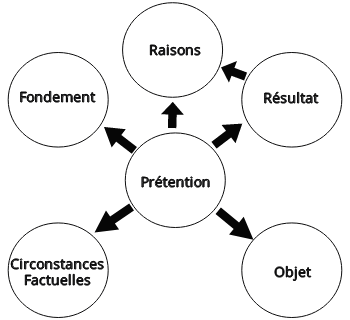
\includegraphics[scale=0.75]{demande-central.png}
    \caption{La demande au centre de l'analyse des décisions}
    \label{fig:intro:demande-central}
\end{figure}

En fait, La granularité de l'analyse est affinée jusqu'à la demande car dans une décision, les juges apportent une réponse à chaque demande, et par conséquent une partie peut voir certaines de ses demandes acceptées complètement, lorsque d'autres accordées partiellement, et le reste est rejetée.  Ceci revoit en effet les modélisations prédictives qui ne s'attardaient qu'à déterminer globalement si le plaintif a  gagné ou perdu le procès sans estimer précisement ce que chaque partie a obtenu. Un juriste sera donc plus intéressé à formuler les demandes qui ont de meilleures chances d'être acceptées qu'à prévoir une victoire du procès. Par ailleurs, les juristes s'intéressent généralement à un type de contentieux à la fois et surtout à des types particuliers de demandes s'appuyant sur une règle ou un principe juridique appelé "fondement". Ainsi, une analyse devrait se faire dans un contexte bien précis, défini par ces différents concepts.


Le problème posé dans notre cas vise principalement l'élaboration d'un modèle prédictif de conséquences judiciaires par l'analyse de jurisprudence. Plus précisément, comment peut-on partir de la jurisprudence d'un type de demande et anticiper le verdict des juges? L'approche est simple: retrouver les décisions portant sur des demandes du type considéré, puis les analyser pour trouver les raisons potentielles pour lesquelles les juges ont pris telle ou telle autre décision. C'est une approche qu'exercent régulièrement les tribunaux pour résoudre de nouveaux jugements, et les avocats et chercheurs pour connaître la pratique judiciaire et donc l'interprétation de la loi généralement adoptée par les tribunaux.

%\textcolor{red}{Description d'une approche traditionnelle, exemple d'études, difficultés de ces études}

L'approche traditionnelle d'analyse d'un contentieux ou d'une demande \citep{ancel2003expulsion} consiste à :
\begin{enumerate}
\item \textbf{choisir un échantillon représentatif}: collection des décisions suivant des contraintes définies:  période précise et d'une couverture géographique, types d'affaires (types d' évidents et types marginaux), diversité, hétérogénéité. 
\item \textbf{Sélectionner les décisions}: élimination des décisions qui ne correspondent pas au type de demande d'intérêt.
\item \textbf{Elaborer la grille d'analyse}: création d'un modèle de grille (tableau) qui permettra d'enregistrer les informations "potentiellement importantes". Chaque ligne correspond à une demande et les colonnes sont les différents types d'informations qu'on peut extraire sur une demande. Ces variables vont de la procédure suivie, aux solutions proposées en passant par la nature de l'affaire. Les champs à remplir ne sont pas connus à l'avance; c'est la lecture des décisions qu'on retrouve les informations qui paraissent intéressant à observer.
\item \textbf{L'analyse des décisions et l'interprétation des informations}: saisie des décisions et statistique sur un logiciel tableur comme MS Excel pour généralement observer la répartition des décisions suivant.
\end{enumerate}

Les longs délais (distance entre l'état capté et l'état actuel) et l'impossibilité d'observer l'évolution des pratiques dans le temps et dans l'espace sont les principales limites de cette approche \citep{ancel2003expulsion}.

Nous traitons d'un sujet en forte relation avec d'autres domaines dont notamment l'analyse économique du droit en ce sens que les informations que notre système extrait faciliteront et accéléreront les analyses empirique menées par les économistes. Nous avons pour exemple, l'analyse empirique des déterminants de la fixation de pensions alimentaires pour enfant lors de divorce réalisée par l'équipe de Bruno Jeandidier \citep{jeandidier2006pensions}. Cette analyse a duré 9 mois pour l'extraction manuelle des informations et la modélisation par régression de la relation entre les déterminant extraits et les pensions alimentaires accordées. L'automatisation est destinée à alléger les méthodes traditionnels de remplissage des grilles d'analyse en extrayant automatiquement les informations pertinentes.

Les travaux de cette thèse s'inscrivent dans un projet qui vise, entre autres, l'automatisation de l'analyse empirique des contentieux pour observer de manière exhaustive et synthétique les pratiques judiciaires. L'objectif final est d'obtenir un système capable de fournir une estimation des chances d'obtenir un résultat positif suivant des critère comme la juridiction, le type de demande, ainsi que les faits du contentieux, et d'identifier les facteurs influençant le résultat. Le projet comprend deux phases principales : une phase d'indexation des connaissances de la masse des décisions, suivie d'une phase d'analyse prédictive. La phase d'indexation doit déjà permettre de réaliser automatiquement des analyses descriptives plus exhaustives. Les analyses descriptives consisteront par exemple à comparer le nombre d'acceptations au nombre de rejets, comparer les quanta demandés et accordés, analyser l'évolution temporelle et la différence spatiale de la prise de décision dans les juridictions. Par conséquent, le système doit apprendre à reconnaître dans les décisions, les informations pertinentes: prétention (partie, objet, fondement) et résultat de la prétention. De plus, les informations extraites doivent s'insérer dans des catégories qui ont un sens en droit. Il y a donc une étape de constitution d'une ontologie des prétentions (réalisée par des experts juriste ou de manière automatisée si possible). Il y a une étape de constitution des bases d'apprentissage et de test pour l'entraînement à la reconnaissance des prétentions et des résultats.
Pour la phase d'analyse prédictive, on doit regrouper des paquets de décisions homogènes (même résultat sur la même prétention dans les circonstances similaires), pour découvrir les facteurs influençant la sens du résultat (par ex. le fait que "le revenu de l'époux soit le plus élevé du foyer" encourage les juges à accorder la pension alimentaire à l'épouse). En effet, c'est la connaissance de ces facteurs permet à l'expert juriste de pouvoir anticiper les décisions judiciaires.

Ce document n'aborde pas l'aspect prédictif du projet. Notre étude s'est limitée aux problématiques liées à l'analyse descriptive et décrites dans la section suivante.

\section{Problématiques techniques soulevées}
\label{sec:intro:probleme}
L'analyse automatique de décisions jurisprudentielles fait références à de nombreux problèmes rencontrés par les juristes lors de leur analyse manuelle (\textcolor{red}{par exemple?}). 

La chaîne de traitement à mettre en \oe uvre consiste en quatre phases principales s'enchainant comme le présente la figure \ref{fig:intro:pipeline-globale}. Les problématiques relatives à chacune de ces phases sont détaillées dans les sous-sections suivantes.
\begin{figure}[h]
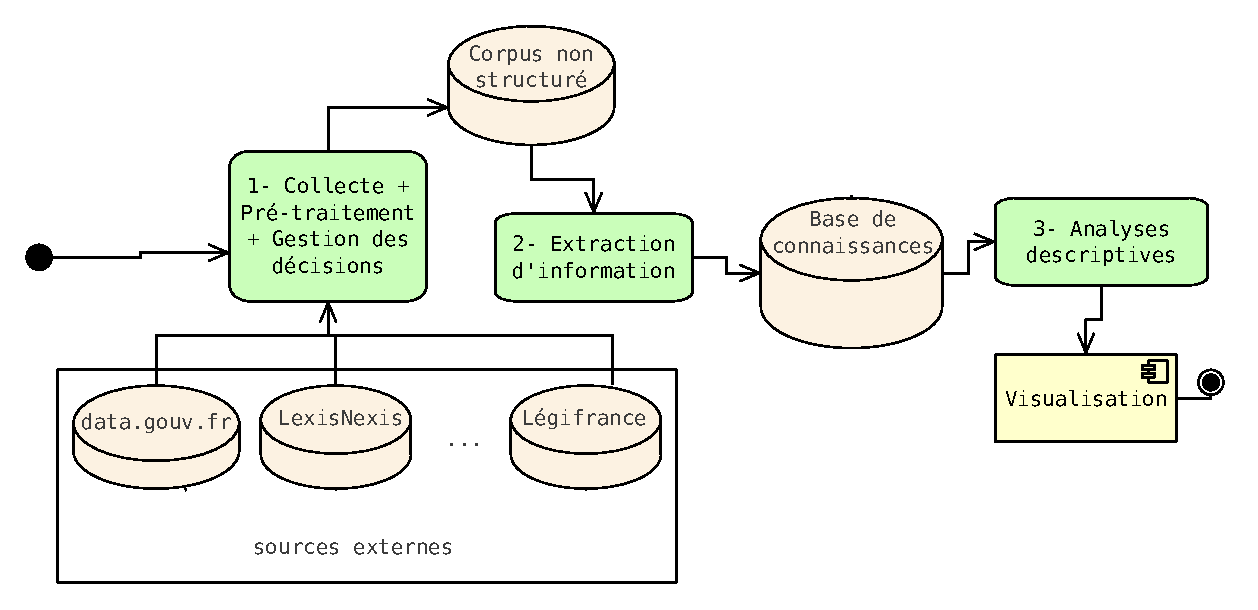
\includegraphics[width=\textwidth]{pipeline-cassandra.pdf}
\caption{Chaine d'analyse du corpus jurisprudentiel à mettre en \oe uvre} \label{fig:intro:pipeline-globale}
\end{figure} 

Dans le cadre de notre travail, nous avons définie et traité les quelques problèmes principaux décrits dans les sous-sections suivantes.

\subsection{Collecte, gestion et pré-traitement des données}

Malgré le fait que les décisions de justice civile sont les premières visées, ce projet a l'ambition de couvrir la majorité des juridictions des 1er et 2nd degrés. Le volume de décisions prononcées est énorme et croit très rapidement mais pratiquement de manière constante (table \ref{tab:intro:nbdecisionstats}).

Les décisions de cours d'appel de la justice civile sont les plus accessibles à travers les moteurs de recherche juridique (LexisNexis\textregistered, 
Dalloz\textregistered, LamyLine\textregistered, Legifrance\textregistered, ...) et la grande base de données JURICA de la Cour de cassation. Cependant, l'accès à ces décisions est généralement payant. Le nombre de décisions téléchargeables simultanément est très faibles sur les sites payants (généralement 20 décisions au maximum). En plus, au bout d'un certain nombre de téléchargements, les sites se bloquent automatiquement. La base JURICA forunit la plus grosse base de décisions de cours d'appel (justice civile) en France. Elle est gérée par la Cour de cassation. L'accès à cette base est offert par Le service de documentation, des études et du rapport\footnote{\url{https://www.courdecassation.fr/institution_1/composition_56/etudes_rapport_28.html}} (SDER). Cet accès est payant pour les professionnels et gratuit pour les universités et centres de recherche en partenariat avec le SDER (moyennant un accord de partenariat). L'accès public et gratuit est fourni principalement par Legifrance, le moteur de recherche juridique du ministère de la justice. Les décisions y sont identifiées à l'aide de numéros consécutifs et accessibles à partir d'un service web à l'aide d'une requête GET du protocole HTTP. Ainsi, à l'aide d'une boucle, il est possible de programmer un client web capable de télécharger l'ensemble des décisions de Legifrance. LegiFrance a cet avantage de proposer des décisions de tous les ordres et de tous les degrés. Cependant, les décisions des juridictions du 1er restent plus rares sur internet et pincipalement disponibles auprès des tribunaux et autres juridictions de premier jugement.

Les décisions existent sous divers formats PDF, DOC, DOCX, RTF, TXT, XML,... Il arrive parfois qu'un fichier téléchargé comprenne plusieurs décisions. Les décisions sont collectées à partir de diverses sources peuvant contenir des documents similaires. Le stockage des documents originaux pose ainsi le problème de redondance et d'identification des décisions. \textit{Comment savoir qu'une nouvelle décision existe déjà ou pas dans le corpus constitué?}. D'autre part, certains moteurs de recherche fournissent souvent des résumés de décisions à la place du contenu original des décisions. Il est important de les supprimer du corpus. Un système de gestion des données collectées est donc nécessaire pour identifier et stocker efficacement les décisions avant que tout traitement d'extraction d'information ne leur soit appliqué.

\subsection{Extraction d'information}

\subsection{Standardisation et représentation des données}
La phase de représentation des connaissances porte sur la structuration effective des décisions dans la base de connaissance. Il est nécessaire de définir préalablement un schéma des données/connaissances qui permettra d'expliciter les éléments et les relations à enregistrer, et le type de requête qu'on peut effectuer sur la base. Ce schéma définit en fait les types de concepts et de liens dont les instances sont les informations extraites des textes.

D'autre part, la base doit avoir une représentation qui permette de la connectée à des bases externes pour élargir les analyses possibles (par ex. l'observation de la distribution de décisions par région/département nécessite de savoir à quelle région/département appartient chaque ville de la base, mais cette information est absente des textes).

\subsection{Recherche d'information ou analyse descriptive}
Comment retrouver des décisions similaires à une situation donnée exprimée à l'aide d'un formulaire ou d'une description en langage naturel? La structuration du corpus permet de sélectionner les critères ou propriétés du type d'affaires qu'on veut analyser. Pour permettre une plus grande expressivité de la situation, on pourrait envisager le cas où un particulier, par exemple, voudrait décrire son problème de manière naturelle à l'aide de phrases\footnote{Exemple de situation décrite en langage naturel: \url{http://www.documentissime.fr/questions-droit/question-46724-emprunt-et-divorce.html}}. L'objectif serait dans un premier temps de retrouver les décisions de la base de connaissances qui paraissent similaires à la situation décrite. Ensuite, l'utilisateur  peut s'aider des modèles prédictifs pour effectuer des analyses.

L'automatisation réussi-t-elle à combler les limites de l'approche traditionnelle (par ex. observation de l'évolution des pratiques judiciaires dans le temps).

On s'attend à ce que les catégories de situations (d'affaires) soient suggérées de manière non supervisée par regroupement automatique (hiérarchique si possible). Après avoir filtrer les demandes suivant les catégories prédéfinies de demandes, il faudrait suggérer des catégories de faits pour regrouper de manières non supervisée les décisions (demandes) des demandes sélectionnées. Avec une structuration fine, on pourrait voir si avec seulement les faits on y arrive ou si on on a besoin de tout le texte.


\section{Méthodologie}
\label{sec:intro:methodologie}
%Proposition d'approches taillées sur mesure et conçues par combinaison et adaptation des techniques établies de la la bibliographie.


Les problématiques propres aux textes juridiques trouvent généralement des analogies avec les problématiques de recherche en analyse de données textuelles. Ainsi l'énorme progrès réalisé dans ce domaine a permis d'obtenir de nombreuses approches transposable au textes juridiques. Cependant, l'adaptation est généralement nécessaire pour obtenir des résultats de bonne qualité hors des domaines pour lesquels ces approches ont été développées \citep{Waltl2016lexia}. De plus, la recherche en analyse de données se fait sur des données qui n'illustrent généralement pas la réelle complexité des données réelles. Etant donné que nous avons effectué l'une des premières études d'analyse de jugements français, nous avons axé notre travail sur le rapprochement des problématiques techniques liées à l'analyse des décisions jurisprudentielles aux problématiques généralement traitées en analyse de données textuelles en général. Il s'agissait ensuite d'établir des protocole d'évaluation et d'annotations nécessaires de données nécessaires. Selon les problématiques identifiées et les protocoles d'évaluations définies, des techniques établies de la littérature ont été adaptés et expérimentés sur les données réelles annotées par des experts.

\section{Résultats}
\label{sec:intro:résultats}
Le projet vise à fournir des outils d'extraction d'information afin de contribuer à la création de nouvelles vues, perspectives et représentations des décisions de justices. Ces outils doivent plus distinctement permettre d'analyser de manière descriptive et prédictive, résumer dans une structure sémantique propre au domaine judiciaire, explorer, visualiser en terme de différence spatiale et d'évolution temporelle, l'énorme corpus de décisions jurisprudentielles qui croit rapidement d'année en année.

\section{Structure du mémoire}
\label{sec:intro:organisation}

\textbf{Chapitre \ref{chap:literature}} \\[0.2em]
%blindtext

\textbf{Chapitre \ref{chap:structuration}} \\[0.2em]
%\blindtext

\textbf{Chapitre \ref{chap:quanta}} \\[0.2em]
%\blindtext

\textbf{Chapitre \ref{chap:sensresultat}} \\[0.2em]
%\blindtext

\textbf{Chapitre \ref{chap:similarite}} \\[0.2em]
%\blindtext

\textbf{Chapitre \ref{chap:conclusion}} \\[0.2em]

\textbf{Les annexes \ref{chap:demo}} \\[0.2em]
